\documentclass[a4paper]{article}
\usepackage{array}  
\usepackage{graphicx}
\graphicspath{ {./images/} }
\usepackage[table]{xcolor}% http://ctan.org/pkg/xcolor
\usepackage{geometry}
\geometry{margin=1.25in}
\usepackage{hhline}
\usepackage{environ}
\usepackage{longtable}
 %\geometry{
 %a4paper,z
 %total={170mm,257mm},
 %left=40mm,
 %right=40mm
 %}
 \newcommand{\colWidth}{141mm}

\begin{document} 
\section*{Demo day: \textit{(Demo 4)} Group \textit{(11 - FE.ED)}}

% ------------GOALS----------

\begin{center}
\begin{tabular}{|p{\colWidth}|}
	\hline
	\cellcolor{blue!25}\large
	\textbf{What were your goals?}
	\\ \hline
	\vtop to 130mm{
	Our goals this time involved our sensors interacting with the environment. We categorised our goals into 3 main areas, the robotics, server and  web app.
    Our goals for each were as follows:
    
    \vspace{8mm}

\begin{tabular}{ ||p{9cm}|p {3cm}|| } 
 \hline \hline
 \textbf{Robotics Goals} & \textbf{Status}   \\ \hline
  \textbf{Camera Rotating}:
  With left and right buttons on the app, this allows the user to rotate the camera, allowing them to see their pet better 
  & Achieved   \\ \hline
\textbf{Weight sensors in the food bowls}: Allows users to monitor daily food consumption of pets. Food containers open up in bursts until the desired amount of food is met.
 & Achieved \\  \hline
 \textbf{3d print food containers } : These food containers allow users to fill up the containers  
 & Achieved \\ \hline
 \textbf{Robot re-designed}:We’ve redesigned chutes and the slide to allow food to be dispenser in a better way  & Achieved \\ \hline
  \textbf{Laser Pointer}:We've added a laser pointer to the camera to allow the owner to play with their pet & Achieved \\ \hline
  \textbf{Bluetooth}: Added Bluetooth to allow users to differentiate pets & Achieved \\ 
 \hline \hline
\end{tabular}

\vspace{ 5mm}

\begin{tabular}{ ||p{9cm}|p {3cm}|| } 
 \hline \hline
 \textbf{Server Goals} & \textbf{Status}   \\ \hline
  \textbf{Persists the state of the app for users}:
  Means that schedules, and pet profiles get kept.
  & Achieved   \\ \hline
 \hline \hline
\end{tabular}

\vspace{ 5mm}

\begin{tabular}{ ||p{9cm}|p {3cm}|| } 
 \hline \hline
 \textbf{Web App Goals} & \textbf{Status}   \\ \hline
  \textbf{Refactor the web app}:
 Allows the app to be more robust when communicating with the server and makes it more reliable. Users now know if something goes wrong.
  & Achieved   \\ \hline
  \textbf{Pet analytics}: Allows users to see how much there pet is eating 
 & Achieved \\
 \hline \hline
\end{tabular}

  }
  \\
  \hline
\end{tabular}
\vskip 5mm


% ------------ORGANISATION----------

\begin{tabular}{|p{\colWidth}|}
	\hline
	\cellcolor{blue!25}\large
	\textbf{Summarise how your group organised the workload to achieve your goals.}
	\\ \hline
	\vtop to 100mm{
	
	We used a sprint setup to try and maximise our efficiency at getting tasks done. We broke down our milestones into smaller independent tasks. This allowed us to isolate the specific tasks we needed to do.To try and make communication easier we tried to work together at the same time, whilst this occasionally was a little bit slower than doing it independently.  This meant that there was a some overlap in what we all worked on. In terms of meeting goals this is where people have worked :
	
	\begin{tabular}{ ||p{5cm}|p {5cm}|| } 
 \hline \hline
 \textbf{Robotics Goals} & \textbf{Who ?}   \\ \hline
  Camera Rotating
  
  & Ishan, Nyal, Luc    \\ \hline
Weight sensors in the food bowls
 & Asmita, Ishan, Brodie, Luc \\  \hline
 3d print food containers 
 & Jerry\\ \hline
Robot re-designed  & Jerry, Brodie \\ \hline
Laser Pointer & Kelly, Brodie \\ \hline
Bluetooth & Nyal, Luc \\

 \hline \hline
\end{tabular}
\vspace{5mm}

\begin{tabular}{ ||p{5cm}|p {5cm}|| } 
 \hline \hline
 \textbf{Server Goals} & \textbf{Status}   \\ \hline
  Keeps the state of the app for users:
 
  & Nyal   \\ \hline
 \hline \hline
\end{tabular}

\vspace{5mm}

\begin{tabular}{ ||p{5cm}|p {5cm}|| } 
 \hline \hline
 \textbf{Web App Goals} & \textbf{Status}   \\ \hline
  Refactor the web app:

  & Nyal, Asmita  \\ \hline
 Pet analytics:
 & Ishan, Asmita, Nyal  \\
 \hline \hline
\end{tabular}

  }
  \\
  \hline
\end{tabular}
\vskip 5mm

% ------------ACHIEVEMENTS----------

\begin{tabular}{|p{\colWidth}|}
	\hline
	\cellcolor{blue!25}\large
	\textbf{What were your main achievements?}
	\\ \hline
	\vtop to 60mm{
	
	\begin{itemize}
	    \item Redesigning the robot to make food dispensing more accurate
	    \item Weight sensors in the food bowls 
	    \item Re-factoring the web app 
	    \item Camera rotating 
	    \item Laser pointer 
	    \item 3d print the food containers 
	    \item Bluetooth 
	    \item Pet analytics 
	\end{itemize}

  }
  \\
  \hline
\end{tabular}
\vskip 5mm

% ------------NOT ACHIEVED----------

\begin{tabular}{|p{\colWidth}|}
	\hline
	\cellcolor{blue!25}\large
	\textbf{What did you not achieve? Briefly explain why.}
	\\ \hline
	\vtop to 150mm{
	
	Just due to time constraints, we don't have all the food containers printed out but we do have designs of what they will look like for Friday.
	\vspace{5mm}
	
	Here are some images of the designs we 3d printed :
	
	\vspace{5mm}
	
	 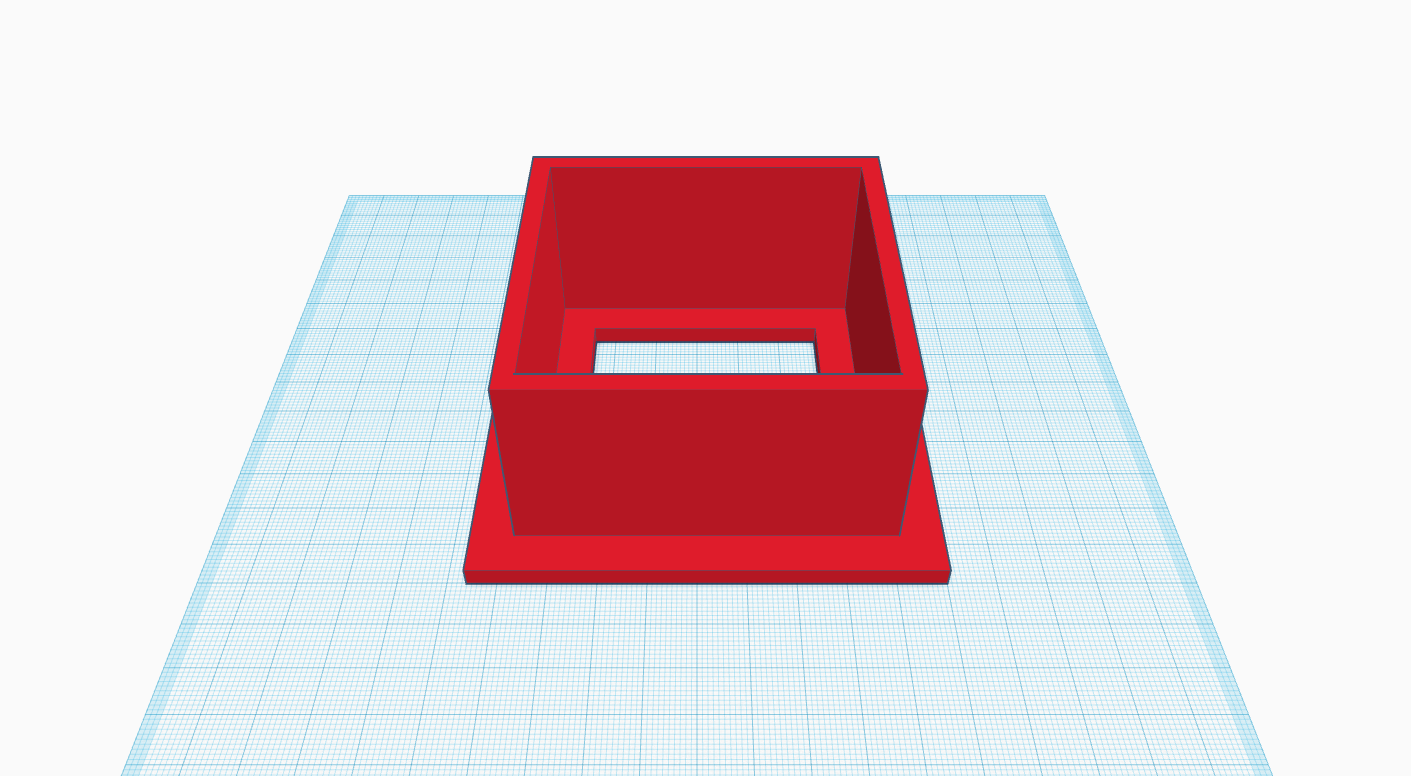
\includegraphics[width=10cm]{image_1.png}
	 
	 \vspace{5mm}
	  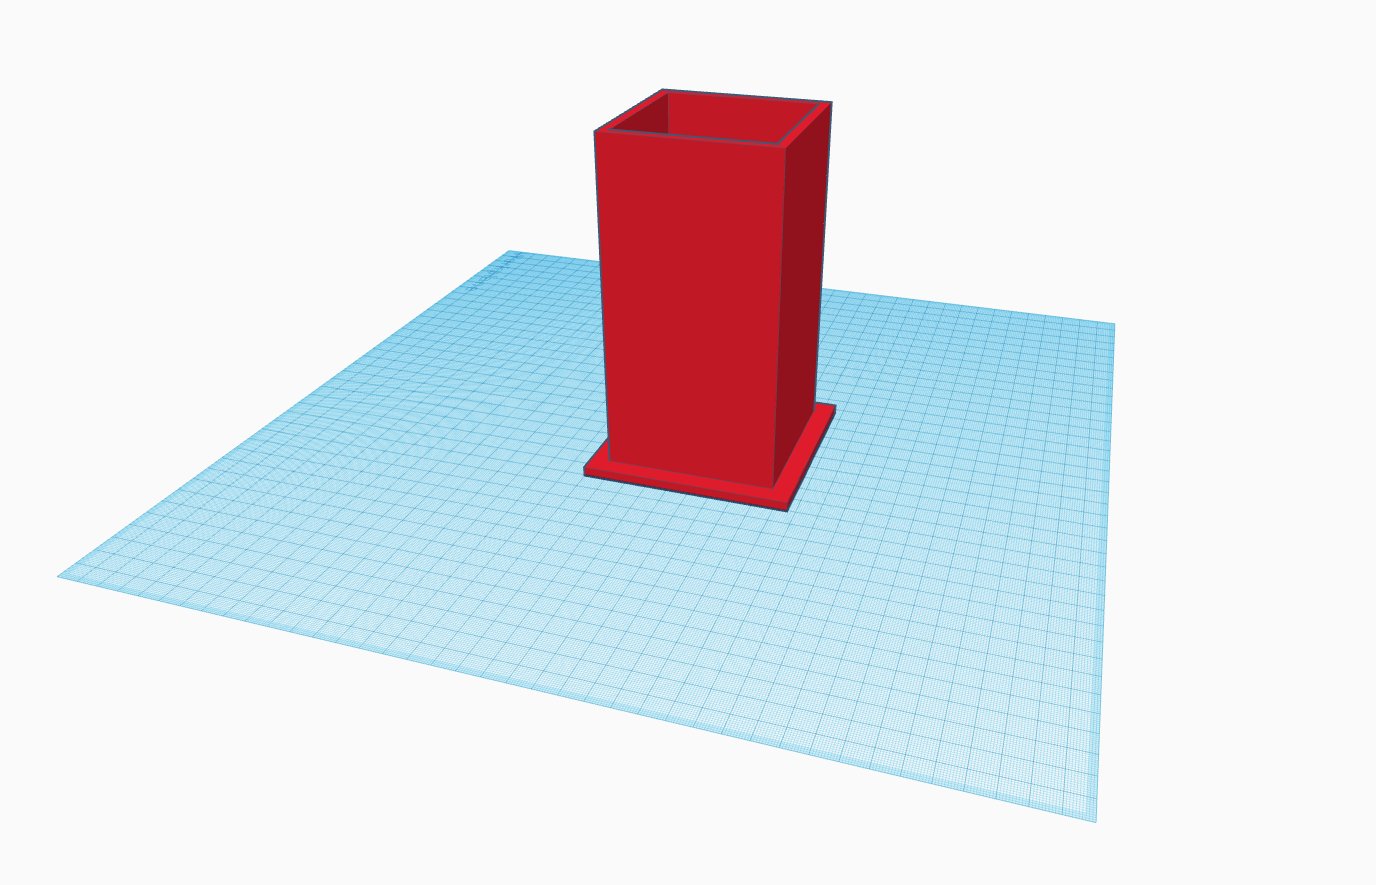
\includegraphics[width=10cm]{image_2.png}
	
	
	
% 	We've also had problems with the weight sensors, which has meant we only have one working.

  }
  \\
  \hline
\end{tabular}
\vskip 5mm

% ------------QUANTITIVE----------

\begin{tabular}{|p{\colWidth}|}
	\hline
	\cellcolor{blue!25}\large
	\textbf{Include any quantitative data you have collected (this can be a graph/table with a few words)}
	\\ \hline
	\vtop to 200mm{

We decided to measure how accurate the weight sensors are. To do this we measured the weight of a small object that weighed 30gs. We proceeded to measured this 40 times placing it on the food bowl every 10 seconds and recording the weight. Below is a frequency chart if the weights recorded:
\vspace{5mm}

 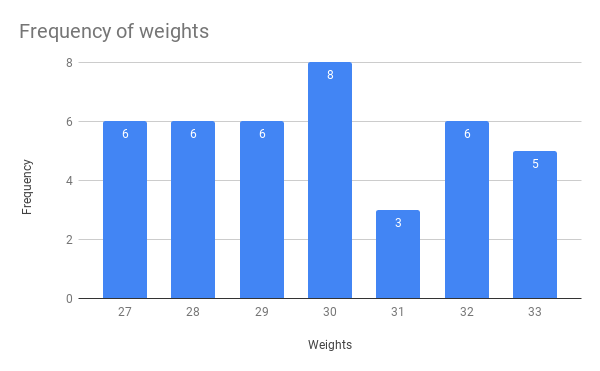
\includegraphics[width=10cm]{weights.png}
 
 \vspace{5mm}
 As you can see the sensor recorded the weight correctly 20\% of the time. We realised there is a margin of error as the weight sensor measures the flex of it and this can change depending on where you place the object on the sensor.
 
 
 \vspace{5mm}
 
 
Camera Rotation testing: This is where we tested how reliable rotating the camera was. Here we decided to test how long it took for the camera to respond. This was to test the lag and how reliable it was. We ran this 35 times. Below is a graph which shows the results:

 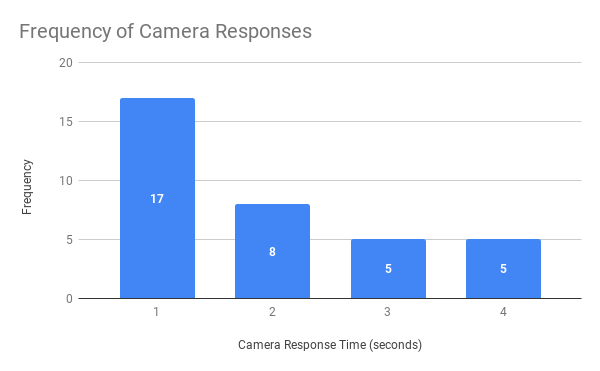
\includegraphics[width=10cm]{camera.png}
 
 From the graph we can see that 48\% of the time it only took one second which is ideally what we would want. This was out of our hands and ideally going forward looking at a motor which responds faster especially with motion recognition is something we would look into.

  }
  \\
  \hline
\end{tabular}
\vskip 5mm

\begin{tabular}{|p{\colWidth}|}
	\hline
	\cellcolor{blue!25}\large
	\textbf{Include any quantitative data you have collected (this can be a graph/table with a few words)}
	\\ \hline
	\vtop to 100mm{

Usability testing:
We've done usability testing on the app to test how easy and intuitive it is to use. We tested this on 15 people by giving them a list of tasks to do and them ranking how easy or hard they found it. 

\begin{itemize}
    \item 100 \% of tasks were done successfully
    \item 93\% found the app easy to use 
\end{itemize}



  }
  \\
  \hline
\end{tabular}
\vskip 5mm
% ------------NEXT STEPS----------

\begin{tabular}{|p{\colWidth}|}
	\hline
	\cellcolor{blue!25}\large
	\textbf{Future for the robot}
	\\ \hline
	\vtop to 45mm{
	
	In terms of the future and scalability  we would use a smaller Bluetooth device so it can be used on a pet's collar just because our design is not feasible for a pet.
	\vspace{5mm}
	
	In terms of object recognition as we have motors turning the camera left and right, the next step with the camera would be to introduce motion detection so that when the pets move the camera can track the pet. (Similar to Mee + Moo)
	
	\vspace{5mm}
	
	Looking into higher quality weight sensors which are more accurate is also something that would be useful to make readings and amounts of food more accurate.
	


}
  \\
  \hline
  
\end{tabular}

\end{center}
  
\end{document}